\chapter{文獻回顧}
\label{chapter:relate-work}

\section{機器人視覺具現化的4個等級}
~\cite{sunderhauf2018limits}提及機器人視覺與電腦視覺領域的主要差異為: 機器人視覺具有具現化(Enbodiment)的能力,這讓機器人可以利用空間或是連續時間的觀察,改善機器人視覺感知的能力。且機器人視覺最後產出的為行動(action) 而非電腦視覺的資訊 (information), 電腦視覺或機器學習常以既有資料集進行訓練, 並著重於資料集的準確度提升, 但機器人視覺可以與環境互動, 則特別關注如何可以藉由機器人與環境互動的方法,讓其更了解環境。在機器人具現化改善感知的難易程度中,共分為4個階層,由易到難依序為連續時間的機器人具現化(temporal embodiment)、空間中的機器人具現化(spatial embodiment)、主動式機器人視覺 (active vision)、主動式操作 (active manipulation)。連續時間的機器人具現化,藉由連續時間的觀察,換句話說以連續圖片作為線索,並假設圖片之間必有緊密之關聯,增加對感知能力的信心指數。空間中的機器人具現是藉由多視角對環境有更深的了解。因為環境常會有遮蔽的狀況,因此透過機器人繞一圈或以不同視角觀察,可以對環境有更強的感知能力。主動式機器人視覺可透過機器人控制移動攝影機, 改變其位置與觀察視角, 藉此得到更多的環境資訊改善優化機器人對環境的感知能力, 改善系統的感知信心指數、解決感知上的歧義、最小化被遮蔽的、反射等問題。主動式操作則是進一步利用會改變場景幫助感知的效果, 例如: 機器手臂可以移動被遮擋的物品得到被隱藏的資訊。這樣的概念被應用於這些研究中: ~\cite{atanasov2014nonmyopic} \cite{doumanoglou2016recovering} \cite{malmir2017deep}採取主動式機器人視覺的概念,採用``next-best viewpoint''的策略改善感知的信心指數,並應用於物件偵測上。
 \cite{zeng2018robotic} 則偏向更高階的主動式操作,採取``grasp-first-then-recognize''策略改善雜亂環境中糟糕的感知效果。
本研究就是藉由主動式操作, 對於商標文字被遮蔽的物件進行操作, 改善對品牌文字及物體的感知能力,進而找出最佳的夾取方法,並進行上架。

\section{夾取成功率預測}
物品夾取成功率(Object affordance )對於機器人操作領域是一個重要的議題。
為了處理雜亂、互相遮蔽的環境、與不同幾何形狀的物品,有許多最新的研究採取同時結合多種演算法並搭配客製化的末端效應器:
~\cite{zeng2016multi}以物體特性及幾何模型定義每一個物品特定的夾取方法,並透過經典的姿態預測:ICP
(Iterative Closest Point) ~\cite{pomerleau2013comparing}找出物件姿態,並決定操作夾取物件的方法。ICP需以點雲資訊匹配三維模型,將實際物體的點雲從
深度攝影機所得到的原始點雲加以分離,才能獲得較好的效果。 因此必須要搭配物體語意分割(Semantic
Segmentation)的方法能夠將物體輪廓較精確的標記,將二維像素分類結果投影
至三維後能得到較單純的物體點雲作為ICP點雲輸入。此外其採用多視角的方法,讓手臂操作攝影機觀察物品數10個角度,並找出一個信心指數最高的姿態,作為感測結果。這個方法雖然有效,但此方法最大的問題在於若有相同物品相鄰時,無法有效切割造成物品姿態預測可能會有問題(圖~\ref{figure:product_vs_bn})。
此外~\cite{zeng2016multi}為了搭配每種物品特定的夾取策略,所使用的夾具乃透過特殊設計,由平行2指夾爪為基底,前端配有可鏟起物品的機構,夾爪上還有可伸縮旋轉的吸盤,提升其夾取效果。此設計可有效提升在針對各種形狀物品在雜亂如靠牆、相鄰情況下,夾取的成功率。雖然可提升夾取成功率,卻難以用特定姿態夾取,且夾爪上也難以進行翻轉,並不適合運用於特定姿態放置的任務。
~\cite{zeng2018robotic}定義4個操作方法(其中2種是以吸盤夾爪夾取,另外2種是以2指夾爪夾取)夾取或吸取物品,並藉由人為標注資料訓練兩個全卷積網路進行像素級別的物品夾取成功率預測。此方法雖能有效率的夾取物品,但卻無法分類物品,需要夾起後再分類。
此外,也有許多研究專門研究使用兩指夾爪夾取物品的物品夾取成功率: \cite{redmon2015real} 以在圖片中只會有一個最佳的夾取姿態的假設,將一張彩色圖片編碼成許多網格(grid cell),並預測最終的夾取位置與姿態。其雖然有效,卻只適合較簡單無遮蔽的場景,若遇到相同物品相鄰的情況,可能會視為同一物品夾取,造成一次夾取兩個物品而失敗。另一方面,在只觀察物體的深度下,~\cite{mahler2017dex}先建立多個候選夾取姿態,並將這些姿態投影到圖片上,並預測這些夾取姿態的夾取成功率以找到最適合的夾取方法。再透過訓練好的深度模型進行預測。排序候選夾取姿態的優先順序。這個方法已證明可夾取多類型的物品。
~\cite{pinto2016supersizing} 採取了多段的學習方法,其融合了卷積網路神經系統(CNN)與強化式學習 (reinforcement learning)學習. \cite{zeng2018learning}透過將兩個平行的全卷積網路(一個專門訓練推,另一個專門旋練夾取)與Q-learning架構,決定現在該進行夾取或是該將原本緊密的物件們先分開再夾取的策略,但目前只有應用於形狀相對容易的積木。以上提出的方法皆有效的改善了雜亂環境與物體互相遮蔽的問題,但卻未考慮到夾取後能否用特定姿勢放置物品。

\begin{figure}[H]
	\centering
	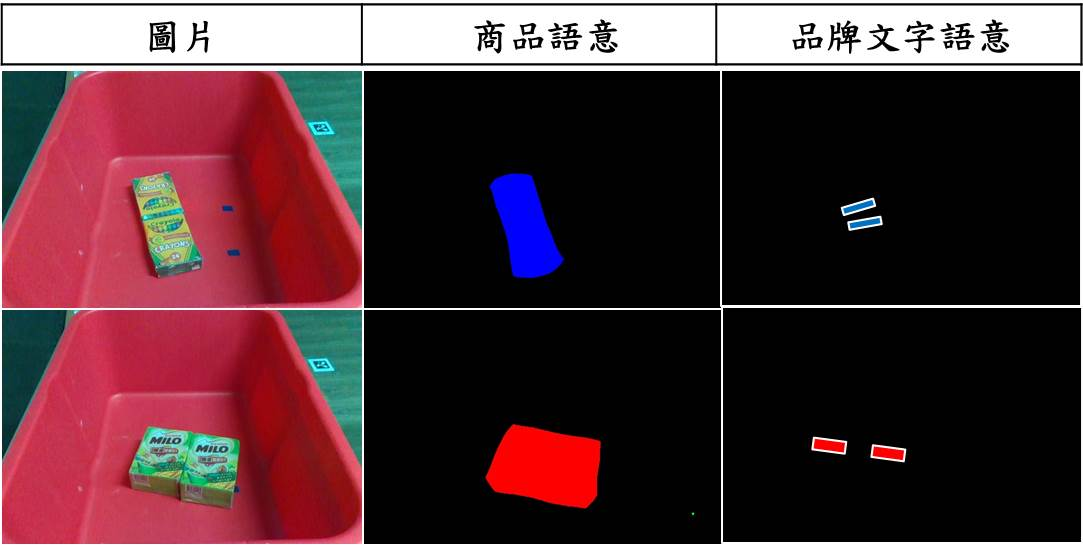
\includegraphics[height=!, width=1.0\linewidth, keepaspectratio=true]
	{./figures/product_vs_bn.jpg}
  \caption{物品語意切割與品牌文字語意切割。物品語意切割在相同物品相鄰時,會無法有效將分開物品,而是將其視為同一物品。但若是只從物品從偵測商品語意如品牌文字等,則可解決這個問題。}
  \label{figure:product_vs_bn}
\end{figure}

\section{雙機械手臂協作}
雖然機器人操作領域的問題已經被大量研究,但都僅限於單隻手臂的情況下, 關於雙手臂操作的應用研究卻較少被關注. 在Smith \textit{et al.} \cite{smith2012dual}研究中,
提出關於雙手臂應用大致可分為兩類:goal-coordinated 方法(在同個環境執行相同任務,但彼此分開行動,無任何合作), 與bimanual manipulation (對同一個物體同時進行操作).
~\cite{schwarz2018fast}便是goal-coordinated approach方法的一個典型例子,其透過兩隻手臂在雜亂盒子裡執行夾取任務,只專注於夾取物品與避免手臂之間互相碰撞,手臂間無合作,
但有效的提升夾取的效率。 而~\cite{harada2012pick} 考慮物品姿態並針對多種形狀物體進行夾取放置任務,系統透過雙手臂執行重夾動作以達到理想的放置姿態。
~\cite{miyazaki2017object}設計一個雙手臂系統,雙手臂各自有不同功能:將物品掃開解決遮蔽問題、使用吸盤夾爪從雜亂的盤子中夾取物體。在Smith分類底下,本研究可被歸類為bimanual: 系統目標處理品牌文字被遮蔽的物品,透過雙手臂(一為使用吸盤夾爪夾取物品至空中以便觀察,二為用2指夾爪穩定夾取並放置物體到架上)。
雙手臂系統可由人形機器人的雙手臂所組成,或者是兩隻獨立的手臂針對特殊需求裝置於不同的平台。上述所提到的~\cite{smith2012dual}屬於後者,由兩隻獨立的手臂所組成,~\cite{schwarz2018fast}~\cite{harada2012pick}屬於前者,裝於人形機器人上。兩者最大的差別在於,透過兩隻獨立的手臂,其空間延展性較大,可活動的範圍較廣。本研究也被分類為由兩隻獨立手臂所組成,活動空間可同時觸及架子以及充滿物體的箱子。

\section{機器人操作領域之基準訓練測試資料集}
在電腦視覺領域,已有許多資料集被作為基準資料庫,如Pascal VOC資料集 ~\cite{everingham2010pascal}共有20類物品,並提供Bounding box與像素集別的標注,供大家用來評估訓練模型的準確度。Freiburg Groceries資料集 ~\cite{jund2016freiburg},則提供5000張常見的日常食用商品,有25個類別共5000張彩色圖片及圖片分類,這些雖都是專門用來評估影像辨識的資料集,並且已受大家公認且大量使用的資料集,但卻與機器人操作無太多關聯。而在機器人操作領域上,目前並無一個公認的資料集做為測試用,但仍有不少研究與此相關:MIT Princeton 團隊所建立的``Shelf \& Tote''資料集~\cite{zeng2016multi}是為了Amazon Picking Challenge,所建立的資料集,此資料集針對當中的39類物品,有完整的彩色圖、深度圖、以及像素及別的標注。也有提供競賽時的場景做為測試集。此測試集可有效評估三維姿態辨識的準確度,本研究所建立的資料集,有數個也挑選競賽所用之物品。Yale-CMU-Berkeley資料集~\cite{calli2015benchmarking}則提供77個物品的高解析度彩色圖、深度圖、以及具有高解析度材質(texture)的三維模型。並分為5類(食物、廚房用具類、工具類、形狀類、任務類),並保證這些物品的來源性,希望能作為機器人操作之基準訓練測試資料集。有許多研究如~\cite{mahler2016dex}使用其資料與模型。有研究也專門建置評估夾取姿態好壞的資料集:VisGraB資料集~\cite{kootstra2012visgrab}結合了現實與模擬的實驗設定,在現實場景與模擬場景中。使用者可使用這個資料集,在模擬場景中用其所設計的評量標準評估演算法所預測出的夾取姿態可行性高低。本研究參考以上許多研究作法,最後採用多視角的自動資料蒐集方式,並同時從虛擬與現實蒐集與標注資料。衡量標準則分別採用真實世界測試集場域評估夾取可行性與商品語意切割準確度。

\section{深度學習物件偵測與辨識}
許多應用場合,在處理深度神經網路上,能夠更迅速並即時的達成工作。在深度神經網路發展中,有許多的應用與影像視覺有關,針對視覺方面的研究,深
度神經網路有一類架構被稱為卷積神經網路(Convolution Neural Network),透過監督式學習給予網路輸入影像及對應的輸出標籤,可以使其自動地學習影像中的
特徵,且隨著卷積神經網路架構不斷地加深,使得深度學習相較於傳統方法更加的準確。其中,在眾多卷積神經網路裡,最具代表性的架構如: AlexNet ~\cite{krizhevsky2012imagenet}以及 VGGNet ~\cite{simonyan2014very},主要用於提取圖像特徵,進而辨識物件。VGG 團隊根據先前開發的類神經網路,將以往神經架構裡較大的
卷積核(Kernal size)改良為較小的尺寸,藉此讓整體的神經架構變得更深,有 16層的 VGG16 與 19 層的 VGG19,原因是多層非線性層可以的學習更多更複雜的
圖像特徵進而提升準確度,且需要的運算量也相對減少。這也讓 VGGNet 成為當時用於辨識物件的類神經網路中,效果及速度皆優於以往的神經網路,儘管
到現今也常被大家所使用。從 VGG 設計理念可以發現,隨著神經網路深度增加,神經網路的準確度應該要提升,但實際卻不是,原因是深度增加會讓神經
元在進行反向傳播(Back propagation)時,讓後面神經層的梯度消失,導致整個神經網路學習失效。而 ResNet ~\cite{he2016deep}設計出殘差模組(Residual block),概念類似於電路短路(Shortcut)的方式,保留層層之間的梯度,藉此設計出比以往更深的神經架
構,分別有 34、50、101、152 層的 ResNet [8],且準確度遠比以往的神經網路還要更高。與分類模型相關的還有VGG-DICTNET ~\cite{jaderberg2014deep
},VGG-DICTNET是一個文字分類模型,並以800,000張由電腦圖學方式所生成的文字圖片,可以用來分類88,172個字典出現過的文字。

而全卷積網路 (Fully Convolutional Network) ~\cite{long2015fully},不同於以往將輸入的圖像做分類,主要是找出圖像中物件的語意分割,實現的方法就是將圖像中每一
個像素(pixel)做分類,也就是像素級別上的預測(pixelwise),使用全卷積網路的好處是可以得到圖像中輪廓分明的物件,但由於整個神經網路需要的運算量
過大,因此計算時間相較於其他神經網路要來的慢,辨識的禎數大約為 2~5 fps(frames per second),較不適用於自駕車即時的辨識,但卻適用於機器人操作上。而YOLO ~\cite{redmon2017yolo9000} 與 SSD ~\cite{liu2016ssd} 一樣也是辨識物件在圖像中的位置,不過是以邊界框(Bounding Box)作為模型輸出。本研究參考全卷積網路架構,修改VGG-16與VGG-DICTNET架構,得到像素集別的語意切割模型。

\section{品牌文字語意切割與姿態預測}
許多發展很久的以物件為單元的物件偵測器可以產生邊界框(Bounding Box)框住物體,這樣的方法不足以解決考慮特定姿態放置的問題。~\cite{peterthesis}使用品牌文字作為線索處理物件姿態的問題。優點是文字以閱讀上來說本身便具有方向性,且文字有其規律性。因此利用品牌文字姿態(文字方向作為X軸、文字平面法向量作為Z軸)定義物件姿態,並使用全卷積網路架構FCN-VGG-DICTNET訓練模型,偵測具旋轉差異性的品牌文字。換句話說,當品牌文字與圖片水平線夾角介於-45$^{\circ}$ $\sim$ 45$^{\circ}$ 之間,才偵測的出來。透過旋轉圖片4次(0$^{\circ}$、90$^{\circ}$、180$^{\circ}$、270$^{\circ}$)方式再進行預測,預訓練模型可達到在任何角度都能找到具旋轉差異性的遮罩,利用此遮罩與點雲的結合,並基於品牌文字姿態的定義(文字方向作為X軸、文字平面法向量作為Z軸)進行計算姿態(圖~\ref{figure:text-pose-extimation-pipeline})。此演算法雖可有效預測品牌文字姿態,間接推得物品姿態,但只可使用於品牌文字可視的情況。本研究參考此演算法設計夾取可行性系統與雙手臂主動式操作系統,可在雜亂環境下,無論品牌文字是否可視,皆可有效夾取並以特定姿態放置物品。

\begin{figure}[H]
	\centering
	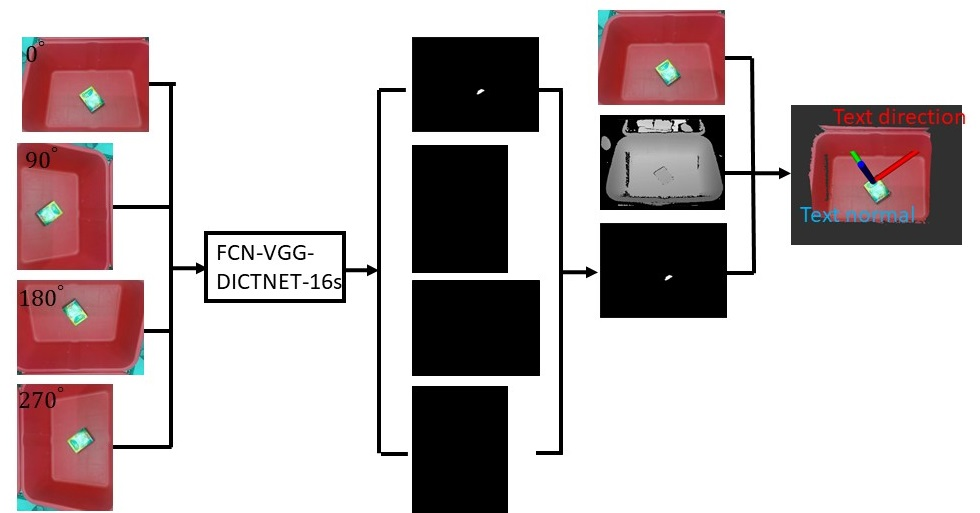
\includegraphics[height=!, width=1.0\linewidth, keepaspectratio=true]
	{./figures/text-pose-extimation-pipeline.jpg}
  \caption{基於品牌文字之語意切割與姿態預測流程圖}
  \label{figure:text-pose-extimation-pipeline}
\end{figure}
